%!TEX TS-program = xelatex
%!TEX root = ../../maxwell2018thesis.tex

\chapter[A Background of Stopping in IIR]{Stopping in Interactive\\Information Retrieval}\label{chap:stopping_background}
Towards the end of Chapter~\ref{chap:ir_background}, we examined a number of different evaluation measures typically employed in~\gls{acr:ir} and~\gls{acr:iir} studies. In particular, we emphasised the notion of different \emph{stopping models} that are implicitly encoded within these measures, ranging from the na\"{i}ve to representative approaches encapsulating a real-world searcher's \emph{stopping behaviours.}

\begin{figure}[h]
    \centering
    \vspace{4mm}
    \resizebox{1\hsize}{!}{
    
\includegraphics{figures/ch3-stopsign.pdf}}
    \label{fig:stopsign}
    \vspace{-5mm}
\end{figure}

In this chapter, we provide an overview of work undertaken in the field of~\gls{acr:iir} that examines the stopping behaviours of searchers. We enumerate on a number of different \emph{stopping heuristics} that attempt to quantify when searchers should stop examining results, before examining \emph{theoretical frameworks} that provide insight and explanation into why and when searchers stop. We then examine a number of different \emph{user studies} that have examined stopping behaviour. Before examining these prior works, we first consider why examining the stopping behaviour of searchers is important to the field, and to the future development of the retrieval systems and their interfaces that we use extensively today.

\section{Why Stopping?}\label{sec:stopping_background:why}
Knowing when to stop is a fundamental aspect of human thinking and behaviour. Humans and other animals when interacting with the world will employ some form of \emph{stopping criterion} to decide when they should stop~\citep{nickles1995judgment}. As an example, a shopper who is looking to purchase a new smartphone will stop shopping around once he or she has obtained sufficient information on what new smartphone to purchase. Once their case notes for a patient have been compiled, a medical doctor will then be in a position to diagnose the patient's ailment. In the context of search, numerous reasons exist why searchers stop -- perhaps because they have satisfied their information need, have become frustrated with the lack of potentially relevant information, or because of some external factor, such as a time constraint that has been imposed upon them.

The decision of when to stop is not exclusively due to such external factors to the decision maker, but rather from a series of \emph{internal, cognitive factors} of their thinking process~\citep{nickles1995judgment}. For example, an individual who is hungry will stop eating once he or she is no longer hungry, rather than stopping when all of the food presented to him or her has been consumed. Empirical research has over the years demonstrated that individuals, regardless of the task presented to them, will frequently stop prematurely. Indeed, this na\"{i}ve behaviour demonstrates that individuals may be willing to go with what \emph{``sounds right''} to them -- often minimising the cognitive effort that is required at the expense of greater accuracy~\citep{perkins1983difficulties}. However, when searching, this lower level of potential accuracy does lead to individuals making a greater number of errors in their decision making~\citep{baron1988heuristics}. Searchers overlook important elements, and potentially miss out useful information~\citep{fischhoff1977cost_benefit, fischhoff1978fault, shafir1992thinking}, with the individual then failing to consider alternatives~\citep{farquhar1993decision_structuring}.

Based upon prior research into stopping behaviour, it is clear that such a decision is driven primarily from internal factors. As such, we then consider: \emph{what aspects of the decision maker's thinking processes prompt him or her to stop assessing the information provided?} Knowing when to stop requires that the individual in question makes a \emph{judgement} regarding the sufficiency of the information obtained, and whether or not additional information is required to be obtained~\citep{browne2004stopping_rules}. This judgement is normally characterised by both the completeness and correctness of the information obtained thus far~\citep{smith1991belief}. These claims can be mirrored by qualitative studies on examining stopping behaviour. Here, researchers have found that searchers stop examining search results simply because what they have found previously is \emph{``good enough''}~\citep{zach2005enough_is_enough} to satisfy their underlying information need. This finding echoes the reasoning that individuals would be happy to stop when what they have found \emph{``sounds right''}~\citep{perkins1983difficulties}.

\begin{figure}[t!]
    \centering
    \resizebox{1\hsize}{!}{
    \includegraphics{figures/ch3-two_points.pdf}}
    \caption[Three main \emph{stopping decision points}]{Excerpts from various searcher models, highlighting three main \emph{stopping decision points,} various points at which searchers can stop performing a given action. These are illustrated as {\color{dmax_lightblue}blue} diamonds. The three points consider \blueboxbold{1} \emph{\gls{acr:serp} level stopping,} \blueboxbold{2} \emph{result summary level stopping} (often called \emph{snippet level} or \emph{query level stopping}), and \blueboxbold{3} \emph{session level stopping}.}
    \label{fig:model_two_points}
\end{figure}

\subsection{Stopping Decision Points}\label{sec:stopping_background:why:points}
In Section~\ref{sec:ir_background:user:models}, we discussed a number of searcher models that are considered an improvement over the traditional~\gls{acr:trec}-style searcher model, a model that is agnostic of a searcher's interactions. These more advanced models considered two distinct \emph{stopping decision points} that capture specific points during the interaction process where a searcher can stop their current activity, and move onto the next step in the process.

These stopping decision points -- along with a new, third stopping point that we discuss later in this thesis -- are illustrated in an excerpt of a typical searcher model flowchart, as shown in Figure~\ref{fig:model_two_points}. Below, each of the stopping decision points are enumerated.

\vspace*{-4mm}
\begin{itemize}
    \item[\blueboxbold{1}]{\blueboxbold{\gls{acr:serp} Level Stopping} The new stopping decision point in this thesis is the point at which a searcher is presented with a~\gls{acr:serp}, and must make a decision as to whether he or she wishes to \emph{enter} the~\gls{acr:serp} and examine content in detail. We provide background and motivation for the inclusion of this new stopping decision point in \todo{Section~\ref{}}.}
    \item[\blueboxbold{2}]{\blueboxbold{Result Summary Level Stopping} Traditionally called \emph{snippet level stopping} or \emph{query level stopping} in the literature\footnote{The phrase \emph{result summary level stopping} is used in this thesis to avoid confusion with the new~\gls{acr:serp} level stopping decision point, discussed in more depth in \todo{Section~\ref{}}.}, this stopping decision point concerns the depth at which a searcher will stop examining a list of ranked results. After stopping at this point, the searcher can continue the search session by issuing a further query.}
    \item[\blueboxbold{3}]{\blueboxbold{Session Level Stopping} This final stopping decision point considers the point where a searcher will stop their search session in its entirety. As such, this stopping decision point is regarded as \emph{terminal} to the search session.}
\end{itemize}
\vspace*{-4mm}

In particular, session level stopping is considered when a searcher must decide, for example, if they have met their overall search goal, have run out of time or queries, or simply have become so frustrated with a lack of relevant content that they would rather abandon the search. These stopping decision points can be operationalised in a variety of different ways, as we explore in the remainder of this chapter.

\section{Stopping Heuristics}\label{sec:stopping_background:heuristics}
Considering the above, researchers have over a number of decades devised a number of different high level \emph{stopping rules} -- hereafter referred to as \blueboxbold{stopping heuristics} -- as a means of encoding a searcher's aforementioned sense of what is \emph{``good enough''}~\citep{zach2005enough_is_enough} -- or, indeed, what can be considered to be \emph{not good enough,} too.

Stopping heuristics have been investigated in \emph{decision making} research. A number of normative stopping heuristics have been identified. As examples of such heuristics,~\cite{busemeyer1988deferred_decision_making} considered the expected loss from terminating information acquisition.~\cite{kogut1990sunk_costs} examined the expected value of additional information. Other examples of normative stopping heuristics are demonstrated by~\cite{pitz1969information_seeking} and~\cite{busemeyer1988deferred_decision_making}.

However, as outlined by~\cite{browne2004stopping_rules}, these heuristics usually fail to describe the actual cognitive behaviours of the decision makers. Such heuristics often assume that the decision maker must \emph{think ahead} to the final decision of when to stop, enabling them to assess the value of additional information~\citep{busemeyer1988deferred_decision_making}. This is however an inherently difficult task for decision makers to undertake, due to the limited working memory capacity of a human. We are simply unable to hold and evaluate all of the information attained to make a decision considering all possible outcomes~\citep{browne2004stopping_rules}.~\cite{nickles1995judgment} agreed, stating that normative stopping heuristics made implicit assumptions about the mental activities of the decision maker, especially in terms of mental scaling and weighting. No clear cognitive perspective is provided to address the assumptions of the decision maker's thinking.

With these inherent limitations in mind, seminal work in this area was undertaken by~\cite{nickles1995judgment} who provided a broad classification for different explicitly defined stopping heuristics in the literature. These heuristics consider a searcher's cognitive processes, and are considered as either \emph{judgement-based heuristics} and \emph{reasoning-based heuristics.} The heuristics we consider are enumerated below, split across the two aforementioned classifications.

\begin{itemize}
    \item{\darkblueboxbold{Judgement-based Heuristics} These heuristics are defined as when a decision maker maintains some mental threshold along a key dimension, and a running total of the number of occurrences of this measure. More details are provided in Section~\ref{sec:stopping_background:heuristics:judgement}.}
    \begin{itemize}
        \item{\blueboxbold{Satisfaction and Frustration} These heuristics consider a decision maker's satisfaction with what they have found during the course of their search \emph{(satisfaction),} or their tolerance to non-relevance \emph{(frustration).}}
        \item{\blueboxbold{Magnitude Threshold} This heuristic concerns a decision maker's belief that the information that they have found provides sufficient evidence to prompt him or her to stop searching for further information.}
        \item{\blueboxbold{Difference Criterion} This heuristic concerns the notion of whether a decision maker is learning anything new with more documents.}
        \item{\blueboxbold{Single Criterion} A \emph{single criterion} to the decision maker's information need is considered in this stopping heuristic.}
    \end{itemize}
    
    \item{\darkblueboxbold{Reasoning-based Heuristics} This classification of heuristic concerns the \emph{mental representation} of the given topic that a searcher is examining information for.}
    \begin{itemize}
        \item{\blueboxbold{Representational Stability} This stopping heuristic concerns the notion of the decision maker's mental model of the topic, and the \emph{stabilisation point.}}
        \item{\blueboxbold{Propositional Stability} Here, a series of potential conclusions regarding the underlying information need are formed, with these arguments needing to be satisfied to stop.}
        \item{\blueboxbold{The Mental List} A mental list of aspects is constructed, with each item on the list needing to be addressed by the decision maker before stopping occurs.}
    \end{itemize}
\end{itemize}

These were devised largely as ways of modelling the~\glsfirst{acr:esl}~\citep{cooper1968expected_search_length}, as briefly discussed in Section~\ref{sec:ir_background:evaluation:system:esl}.~\cite{nickles1995judgment} also proposed a number of stopping heuristics that are discussed in subsequent sections, with discussion expanded to included additional heuristics defined by other researchers. We now address each of the two classifications in turn, explaining each of the different heuristics enumerated above in detail.

\subsection{Judgement-Based Heuristics}\label{sec:stopping_background:heuristics:judgement}
As discussed previously, a judgement-based stopping heuristic is defined as when a decision maker is assumed to set and consistently maintain a mental threshold along some form of key dimension (e.g. determining the seemingly relevant from non-relevant), and to keep a running total of measure relative to the dimension in question~\citep{gettys1979hypothesis, nickles1995judgment}. When the measure is met or exceeded this set threshold, the searcher will then stop their searching activity. Each of the judgement-based heuristics we consider in this thesis are discussed in turn below.

\subsubsection{Satisfaction and Frustration}\label{sec:stopping_background:heuristics:frustration}
Two of the earliest stopping heuristics defined in the literature are by~\cite{cooper1973retrieval_effectiveness_ii} which consider a searcher's tolerance to relevant and non-relevant material. The heuristics were originally defined as a means for estimating the utility a searcher can attain when interacting with a retrieval system. While the means of which~\cite{cooper1973retrieval_effectiveness_ii} estimated the utility of search are not of key relevance to this thesis, the work on stopping heuristics are. The \emph{satisfaction point} and \emph{frustration point} stopping heuristics are considered to be judgement-based heuristics as they rely solely on the searcher's notion of what constitutes a relevant document -- and both consider counts of the number of (non-)relevant documents observed.

\blueboxheader{Satisfaction Point}
Given the name, it is not surprising that the \emph{satisfaction point} heuristic considers the point at which a searcher has found enough perceived relevant material to consider his or her search a success. It can be easily imagined that such a heuristic would apply directly to both result summary level stopping (i.e. \emph{find $x$ relevant documents on this SERP}) and session level stopping (i.e. \emph{find $x$ relevant documents}). This heuristic is also called the \emph{satiation heuristic}~\citep{simon1955satiation} (see below). This heuristic can be considered as a decision making process...

\begin{quote}
    \emph{``[...]through which an individual decides when an alternative approach or solution is sufficient to meet the individuals' desired goals rather than a perfect approach.''}
    \attrib{\cite{simon1971decision}}
\end{quote}

This essentially suggests that a searcher employing this particular heuristic would stop searching as soon as certain conditions arise, instead of after they have exhaustively considered all available information~\citep{march1994primer}. Conditions could include acceptance of the results, discomfort, boredom, time limits and the \emph{snowballing} of information~\citep{mansourian2007search}.

\blueboxheader{Frustration Point}
In a converse fashion to the satisfaction point heuristic, the \emph{frustration point} heuristic considers a searcher's overall \emph{tolerance to non-relevance} by stopping after being sufficiently frustrated by the results presented to the searcher. This heuristic is also called the \emph{disgust heuristic} in the literature (see below).

The two relatively straightforward heuristics defined above makes a searcher's interactions with a ranked list of results \emph{inherently adaptive.} In other words, given a set of results, his or her behaviour will change with respect to the perceived quality of the ranked list. As a reminder, this would not necessarily mean considering the system's effectiveness measures, but rather user-focused measures such as interactive precision and recall, as discussed previously in Section~\ref{sec:ir_background:evaluation:user:ipr}.

\blueboxheader{Combining Satisfaction and Frustration}
Perhaps due to the relative simplicity of two aforementioned heuristics, identical approaches have also been defined elsewhere in the literature.~\cite{kraft1979stopping_rules} later defined three further stopping heuristics, two of which are the \emph{satiation} (as per~\cite{simon1955satiation}) and the somewhat loaded \emph{disgust} heuristics. In essence, the rules defined by~\cite{kraft1979stopping_rules} are the same satisfaction and disgust heuristics as previously defined by~\cite{cooper1973retrieval_effectiveness_ii}. Within the satiation rule, a searcher will stop after been \emph{satiated} by finding a number of documents considered to be relevant, while the disgust rule considers a searcher's disgust at finding a number of non-relevant documents.

\cite{kraft1979stopping_rules} also proposed a third heuristic that \emph{combines} both the satisfaction/satiation and frustration/disgust rules together into a single heuristic. Here, a searcher following such an approach would be inclined to stop examining content if they were either satisfied with what had been found, or frustrated by having to trawl through a number of material judged to be non-relevant. The stopping point would be whatever of the two conditions are met first. Indeed,~\cite{kraft1979stopping_rules} demonstrated that the~\gls{acr:esl} of a searcher could be approximated using each of the two stopping heuristics by considering the size of the retrieval set, the number of relevant documents a searcher wished to obtain, and the number of non-relevant documents a searcher would be willing to tolerate. The number of documents required to consider a search as successful is dependent upon whether the search task is high precision (where one would stop comparatively early) or high recall (where one would stop comparatively later), as hypothesised by~\cite{bates1984thirty_items}.

\subsubsection{Magnitude Threshold}\label{sec:stopping_background:heuristics:magnitude}
\begin{wrapfigure}[11]{r}{0.45\textwidth}
    \begin{center}
    \vspace*{-10mm}
    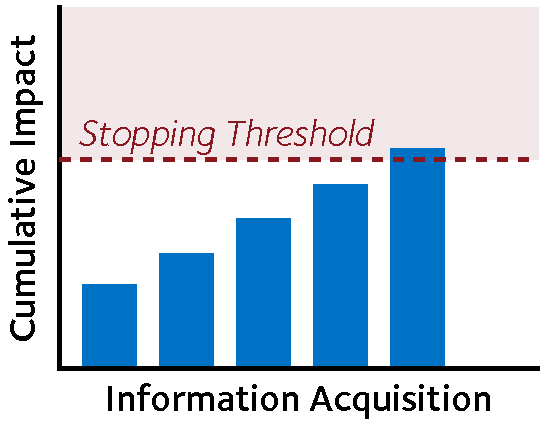
\includegraphics[width=1\textwidth]{figures/ch3-threshold.pdf}
    \end{center}
    \vspace*{-6mm}
    \caption[The magnitude threshold stopping heuristic]{The magnitude threshold heuristic. Once a searcher accrues a predetermined level of impact, he or she stops. Adapted from~\cite{browne2004stopping_rules}.}
    \label{fig:threshold}
\end{wrapfigure}

The magnitude threshold heuristic~\citep{nickles1995judgment} considers an individual's belief that the information accrued during the search process provides \emph{sufficient evidence} to prompt him or her to stop searching for further information. The point at which the searcher would decide to stop is determined by some predetermined, internal threshold that must be reached, which acts as the stopping criterion~\citep{wald1948sequential_analysis, nickles1995judgment}.~\cite{gettys1979hypothesis} hypothesise that the searcher \emph{`mentally tabulates'} the cumulative impact of the evidence that he or she has uncovered, and when the internal tabulation crosses the specified threshold, he or she stops.

Determining what exactly this threshold should be before commencing a task has attracted research from several perspectives. Indeed, this decision can be left open to interpretation by the individuals who choose to operationalise such a heuristic. However, research has shown that under different tasks, varying the criteria by which an individual bases their initial threshold value varies. For example,~\cite{busemeyer1982choice_behaviour} demonstrated this for decision making under uncertainty.~\cite{saad1996stopping} demonstrated the usefulness of this heuristic under common choice tasks.

An abstract representation of the stopping heuristic is provided in Figure~\ref{fig:threshold}. From the figure, we can see that a searcher accrues information through each document that is examined. This is combined together to form a \emph{cumulative impact} of the information. For each document examined, the current cumulative impact value is compared against a predetermined threshold value. If the cumulative impact is above this threshold, the searcher then assumes that enough supporting evidence has been collected, and stops.

\subsubsection{Difference Threshold}\label{sec:stopping_background:heuristics:difference}
The \emph{difference threshold heuristic}~\citep{nickles1995judgment} concerns whether a new document is teaching a searcher anything new about their information need, or the marginal value of the latest document. Here, the searcher is assumed to keep an internal record of the information that has been consumed along some key dimension. The searcher is also assumed to use this internal record of what has been assessed to compare a new document with previously examined content. When the difference between the new and existing information falls below some internal difference threshold, the searcher stops as nothing new is being learnt.

\begin{figure}[t!]
    \centering
    \resizebox{1\hsize}{!}{
    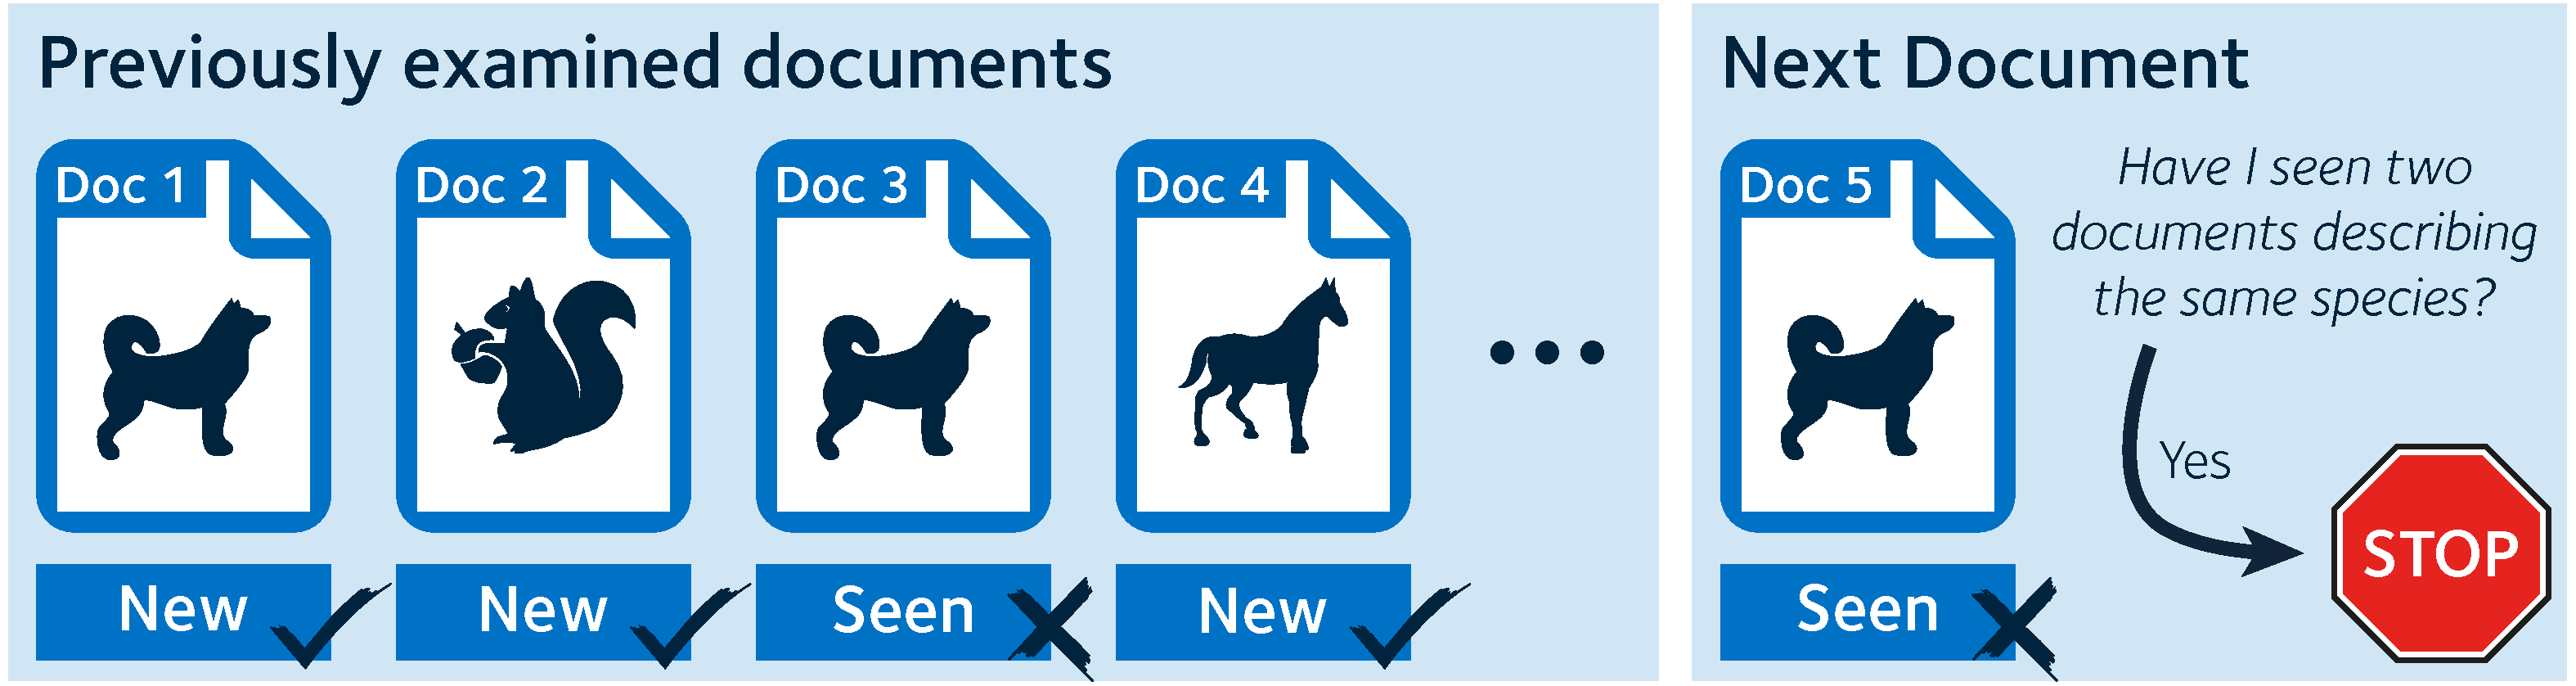
\includegraphics{figures/ch3-difference.pdf}}
    \caption[Difference threshold heuristic]{A simplified, visual example of the difference threshold heuristic. Given the information need of finding different species of animal, a searcher issues a query, and examined a number of documents. The third document offers information on dogs, which has been already observed in \emph{Doc 1.} Using the stopping criterion that once the same species has been observed twice, \emph{Doc 5} satisfies it. This then means that the threshold has been met, and the searcher then stops.}
    \label{fig:difference_heuristic}
\end{figure}

As a crude example of this heuristic, a searcher is provided with an information need to find as many different species of animal as possible. Once a query has been issued, the searcher begins to examine documents on the SERP. This is illustrated in Figure~\ref{fig:difference_heuristic}, where the first document considers dogs. A simple criterion is employed whereby the searcher stops after encountering the same animal twice, illustrating that nothing new is being learnt from the list of results presented. Once this is met, the searcher abandons the SERP, and can then perform a query reformulation to discover different species of animal.

\subsubsection{Single Criterion}\label{sec:stopping_background:heuristics:single}
The \emph{single criterion heuristic} was later defined by~\cite{browne2005stopping_rules}. As the name suggests, this heuristic considers a searcher examining information for a \emph{single criterion} related to their information need, typically assumed to be the most important one. The searcher then stops examining content once he or she has deduced that enough information about said criterion has been accumulated for them to be satisfied. The concept of a stopping threshold can be borrowed from the magnitude threshold heuristic, discussed in Section~\ref{sec:stopping_background:heuristics:magnitude}. This considers that a searcher will stop once they have accumulated enough impactful information.

\cite{browne2005stopping_rules} go on to provide an example search task where the single criterion threshold would be directly applicable. When purchasing a mortgage for a new house, a searcher will explore the websites of various mortgage lenders in order to find the best deal for them. Given a mortgage deal, the most obvious criterion that an individual would look for would be interest rates, with the lower the rate, the more attractive the deal. Of course, other factors may influence the decision, but this example ultimately demonstrates how the heuristic works in simple terms.

\subsection{Reasoning-Based Heuristics}\label{sec:stopping_background:heuristics:reasoning}
The second category of stopping heuristics as defined by~\cite{nickles1995judgment} are \emph{reasoning based}. While searching and accruing information about a particular topic, a searcher is essentially developing a mental representation of the topic~\citep{yates1990decision_making}. As argued by~\cite{nickles1995judgment}, these elements can include arguments constructed during informal reasoning, previously constructed arguments, or information evoked from the searcher's long term memory. As such,~\cite{nickles1995judgment} devised a category of stopping heuristics that are dominated by the searcher's reasoning processes.

\subsubsection{Representational Stability}\label{sec:stopping_background:heuristics:representational}
\begin{wrapfigure}[8]{r}{0.45\textwidth}
    \begin{center}
    \vspace*{-11mm}
    
\includegraphics[width=1\textwidth]{figures/ch3-representational.pdf}
    \end{center}
    \vspace*{-5mm}
    \caption[Representational stability stopping heuristic]{A crude illustration of the representational stability stopping heuristic. The searcher's model of the given information need begins to stabilise at \emph{t-1}, meaning that a searcher would stop at \emph{t}.}
    \label{fig:representational_heuristic}
\end{wrapfigure}

The representational stability heuristic~\citep{nickles1995judgment} (with the phenomenon initially discussed by~\cite{yates1982toward}) concerns the notion that as a searcher acquires new information, his or her mental model of the underlying information need shifts and develops -- but only up to a certain point. From this point onwards, their mental model stabilises and the searcher is said to have accrued enough information to satisfy or understand the (sub)topic.

It is stated by~\cite{nickles1995judgment} that while a searcher examines content, he or she generates arguments that serve to develop and elaborate his or her conception of the decision(s) that they are tasked to make. As the searcher continues to reason, certain arguments may be relegated to long term memory due to the limited size of the searcher's working memory. Searchers will accrue new information, with some perhaps returning to the original subset of arguments. As mentioned previously, it is at this point that can be interpreted as a form of stability regarding the information need. This is depicted in Figure~\ref{fig:representational_heuristic}, where given a vague information need, a searcher will trawl a series of documents in order to develop their mental model of the given problem, turning their understanding of the topic from an initial \emph{fuzzy} state to \emph{crystal clear.}

\subsubsection{Propositional Stability}\label{sec:stopping_background:heuristics:propositional}
Similar to the representational stability heuristic,~\cite{nickles1995judgment} also defined the \emph{propositional stability} heuristic which again focuses on the concept of a stabilising mental model of the given information need. Here, a searcher when examining content will form a series of arguments from the information he or she is observing. These arguments can lead to \emph{tentative conclusions}, from which at some point stability is achieved, and the conclusion does not change. This heuristic therefore suggests that the stabilised nature of the decision maker's conclusion from the information observed prompts him or her to stop.

\subsubsection{The Mental List}\label{sec:stopping_background:heuristics:mental}
The mental list stopping heuristic considers a mental list of aspects of some phenomenon. Each of the different aspects within the mental list must be \emph{`checked off'} to a satisfactory level before the searcher then decides to stop examining content. This mental list can typically be constructed from a searcher's long term memory, meaning that they will likely have \emph{a priori} knowledge of the particular information need. So-called belief structures such as \emph{schemas}~\citep{bartlett1933remembering} or \emph{scripts}~\citep{schank1977scripts} may assist the searcher in organising the construction of the mental list that forms the set of criteria that determines when they stop.

Figure~\ref{fig:mental_list} provides a graphical illustration of the mental list heuristic. When looking for a new car, a searcher will construct a mental list of different aspects of a car which are essentially the minimum requirements (e.g. a minimum engine displacement of 1.8 litres). Searching is then conducted, with the searcher narrowing down the potential choices available to them to those that satisfy their mental list.

\begin{figure}[t!]
    \centering
    \resizebox{1\hsize}{!}{
    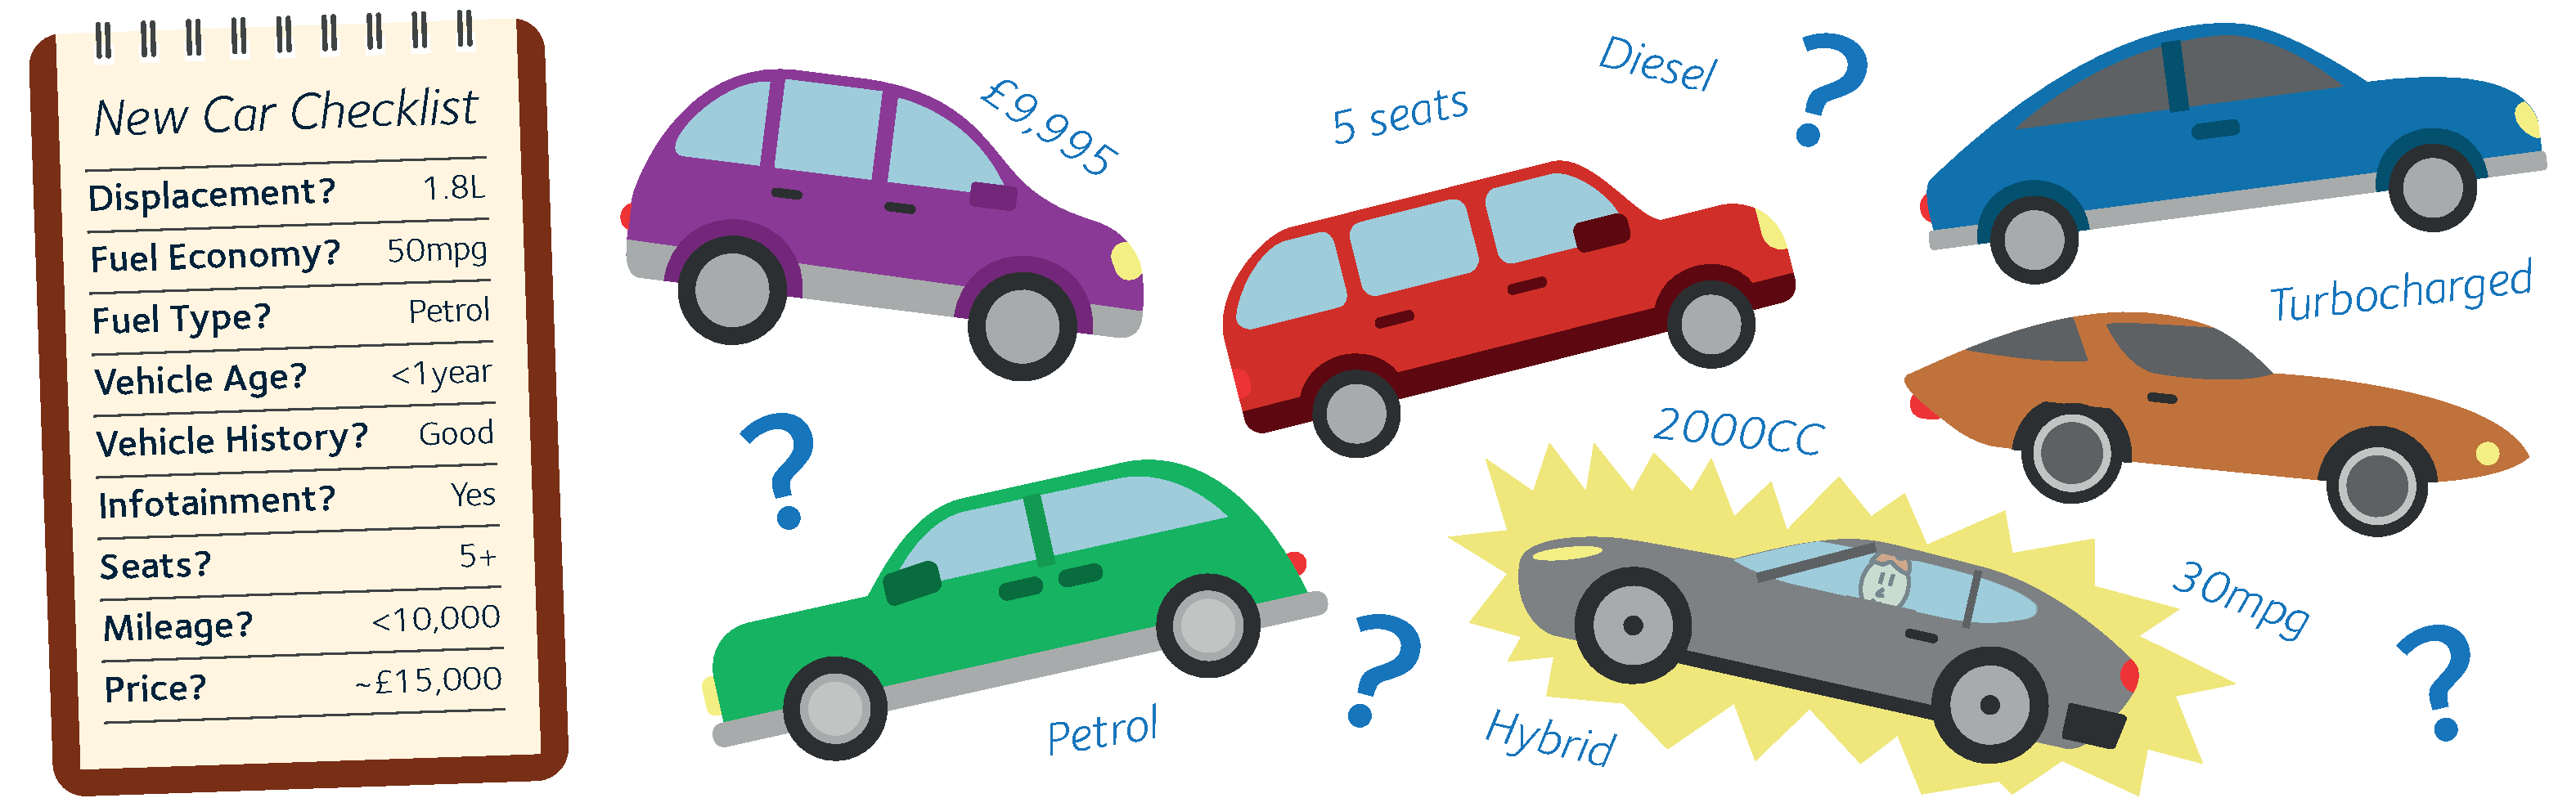
\includegraphics{figures/ch3-mental_list.pdf}}
    \caption[The mental list stopping heuristic]{Given a well defined information need,~\cite{nickles1995judgment} defined the mental list heuristic – where a number of different criteria must be satisfied before stopping. In the illustration above, car shopping is used as an example. Here, certain criteria for a new car (as shown on the notepad) must be met before a searcher is satisfied with what they have found.}
    \label{fig:mental_list}
\end{figure}

\section{Theoretical Models}\label{sec:stopping_background:theoretical}

\subsection{Information Foraging Theory}\label{sec:stopping_background:theoretical:ift}

\subsection{Other Theoretical Models of Search}
Mention~\gls{acr:set}, but only in passing. And then you can say the query cost hypothesis in the later section of the user study.

\subsection{Summary of Heuristics}
In this section, a number of different stopping heuristics have been discussed from a number of seminal papers in the literature. While a much larger of number of normative stopping heuristics have been defined in prior works, these have been omitted from the review as they do not adequately describe the cognitive behaviours of a searcher, often assuming a searcher has to \emph{think ahead} to make a decision to stop or continue~\citep{browne2004stopping_rules}. In contrast, the heuristics that are enumerated above do not make this assumption, making more realistic assumptions about the searcher's cognitive abilities.

Of course, the different stopping heuristics discussed above are likely to behave differently under different search contexts. As an example, the mental list heuristic might be impossible to use given a searcher with a very limited knowledge of a topic. He or she simply would not know enough information to ascertain key aspects of the topic, and construct a set of criteria that must be met~\citep{browne2005stopping_rules} --~\cite{gigerenzer1999betting} also discuss this reasoning for the single criterion heuristic. As such, it is hypothesised that the aforementioned stopping heuristics would be likely to work better with a searcher who is more knowledgeable.

%Indeed,~\cite{browne2005stopping_rules} hypothesises that magnitude threshold and mental list heuristics would be best applied to searchers with a greater degree of understanding of the topic.

\cite{browne2005stopping_rules} also discuss the so-called \emph{``structuredness''} of a given search task. If the task has well defined inputs and outputs -- or the goals and operations are clear and easily understood~\citep{simon1996sciences} -- then it it hypothesised that searchers will employ more precise stopping heuristics for deducing when to stop. For example, the mental list and single criterion stopping heuristics might offer greater degrees of precision than for example the frustration and satisfaction heuristics, although the frustration and satisfaction heuristics may perform well for any given search task. Altogether however, the heuristics discussed in this section would be applicable for informational search tasks~\citep{browne2005stopping_rules}, such as ad-hoc retrieval (refer to Section~\ref{sec:ir_background:paradigms:trec}).

With the heuristics now enumerated, we later in this thesis discuss how we take these stopping heuristics, and consider how to \emph{operationalise} them, such that they can be subsequently implemented and compared against each other empirically. This also involves which of the three stopping decision points we discussed in Section~\ref{sec:stopping_background:why:points} these operationalised heuristics can be used in. \todo{Section~\ref{sec:proposal:strategies}} provides a complete set of the thirteen \emph{stopping strategies} that we employ in the contributory work in this thesis.

\section{User Studies}\label{sec:stopping_background:user_studies}
While stopping heuristics provide a means for quantitatively characterising and predicting stopping behaviour~\citep{wu2014information_scent}, only a handful of user studies have been undertaken that attempt to understand when enough information is enough~\citep{zach2005enough_is_enough}. As we have already discussed, stopping is an inherently difficult phenomenon to model effectively -- this is because it is instrumented by a series of internal factors to the decision maker's thinking~\citep{nickles1995judgment}. In this section, we detail a number of different user studies that have attempted to provide an explanation for a searcher's stopping behaviours.

\subsection{Understanding Stopping Behaviours}
Two user studies by~\cite{zach2005enough_is_enough} and~\cite{berryman2006defines} have reported on an of stopping behaviours through a series of interviews with subjects. These studies primarily focused on the notion of \emph{why} searchers stopped when they did, both considering an academic work environment.

\cite{zach2005enough_is_enough} considered how senior art administrators determined when to stop searching in their daily jobs, and found that they mostly stopped either because they either:

\begin{itemize}
    \item{felt satisfaction with the information that they had obtained during their search;}
    \item{stopped because of time constraints.}
\end{itemize}

The study by~\cite{berryman2006defines} was conducted in a similar vain, where public sector policy workers reported finding it difficult to work out how much information would be enough to satisfy their tasks when initiating them. However, once the structure of what they needed to find has been established, the point at which they felt they should stop became clearer. The findings from this second study provide evidence that the assessments of what constitutes as \emph{enough} can be difficult and complex to deduce. This finding also provides evidence of the development of an underlying mental model of the given information need, and provides justification for the representational stability, propositional stability, and mental list stopping heuristics (as discussed in Section~\ref{sec:stopping_background:heuristics:reasoning}).

A number of user studies have also examined stopping behaviour in relation to the concept of satisfaction or satiation~\citep{simon1955satiation}. As previously discussed in Section~\ref{sec:stopping_background:heuristics:frustration}, this concept suggests that a searcher will cease searching as soon as conditions arise, instead of after they have exhaustively considered all available information~\citep{march1994primer}.

Considering this approach,~\cite{agosto2002satisficing} examined the decision making of young people when searching on the~\gls{acr:www}. In this study, 22 9\textsuperscript{th} and 10\textsuperscript{th} grade students from a U.S. high school demonstrated limitations which affected their decision making, including time constraints that were imposed externally and internally, information overload and other physical constraints. In order to find websites to help in satisfying their information need, the students used reductive approaches to decrease the amount of information presented on the~\gls{acr:www}, and used this to work out when to stop. How students perceived the websites was also largely down to personal preference.

With a completely different set of subjects,~\cite{mansourian2007search} conducted a study where they analysed the stopping behaviours of 37 staff and students from four university biology departments, and classified their stopping behaviours by search depth and search impact. Qualitative results showed that subjects indicated that missing potentially important information in the course of their searching was a matter of concern. The authors reported that the estimations and importance of information missed likely would affect their stopping behaviour. From this, classifications of the perceptions of missing information ranged from \emph{inconsequential} to \emph{disastrous}, and search strategies classified as \emph{perfunctory} to \emph{extensive}, with the information need dictating what category the searcher would have considered appropriate.

A similar study by~\cite{prabha2007enough} considered searchers in a further academic library setting, with one key finding from their study showing that time constraints led to a decrease in the number of documents that searchers examined. Again, the specific information need and the searcher's role in academia affects every stage of their search processes -- which includes affecting what they have found to be enough.

These findings were further demonstrated by~\cite{wu2014information_scent}, who undertook a study where subjects performed a series of different search tasks. Subjects were then interviewed about their query stopping and task stopping behaviours. Results from this study showed that query stopping decisions were taken primarily on the face of search results, queries and search tasks. Task stopping decisions were determined by the subject's overall goal for each task, the content examined -- and their subjective perceptions of the examined content -- and the study constraints imposed upon them, such as time constraints and search interface restrictions. Further empirical evidence to this study was later provided by~\cite{wu2014stopping_query_abandonment}. They reported that some subjects discussed \emph{``forced stopping''} (stopping when no more information could be found), and \emph{``voluntary''} stopping that stemmed from the feeling of securing enough (or a necessary amount of) information.

\cite{wu2014information_scent} also discussed how the \emph{information scent}\footnote{\todo{MOVE THEORETICAL BEFORE THIS} While we discuss \emph{information scent} in more detail in Section~\ref{sec:stopping_background:theoretical:ift}, the scent of a page concerns the strength of the information provided to the searcher, who examine varying \emph{cues} on the page to make a decision. A page yielding a high information scent can therefore be said to contain good quality results that will aid the searcher in satisfying his or her information need.} affects the stopping behaviour of a searcher. Constituting part of~\glsfirst{acr:ift} that we discuss in Section~\ref{sec:stopping_background:theoretical:ift}, it is important to note that user studies have been conducted using this approach. For example,~\cite{card2001scent_graphs} observed that if a person started with a high information scent web page, he or she would visit more web pages at the site. They also found that as the information scent of web pages declined, there was a tendency for the person to leave the site or return to a previously visited page.~\cite{loumakis2011image_smells} examined scent that was associated with images presented on~\glsplural{acr:serp} impacted with the evaluation behaviour of searchers. They found that when images were added to text snippets, participants reported increased confidence that they could find an answer.

Central to the findings of all of the above studies -- regardless of the group of subjects or contexts in which they found themselves to search in -- is the idea that searchers stop when they are \emph{satisfied.} Even though subjects of these studies were acutely aware of the fact they had not found \emph{all} relevant information to their given information need, they were nevertheless satisfied with what they had found, and subsequently decided to stop. While the results from these studies may be underwhelming in terms of concrete explanations as to why people do stop, they do provide invaluable insights -- and demonstrates just how difficult it is to encapsulate such behaviour. Indeed, factors such as time constrains, a searcher's information seeking ability and other factors all influence the internal stopping rules of a searcher, as was discussed by~\cite{marchionini1995information_seeking}. 

\subsection{Quantifying Stopping Behaviours}
With the above studies examining \emph{why} people decide to stop, a very limited number of studies have attempted to quantify \emph{when} a searcher should stop searching -- somewhat akin to the stopping heuristics defined in Section~\ref{sec:stopping_background:heuristics}.~\cite{toms2009predicting_stopping} studied the actions preceding the endpoints in information, seeking to predict what actions would lead a searcher to stop. The most prevalent patten they observed -- that matches the searcher models outlined in Section~\ref{sec:ir_background:user:models} -- consisted of a searcher:

\begin{itemize}
    \item{issuing a query;}
    \item{examining results presented to them on a~\gls{acr:serp}; and}
    \item{viewing a document.}
\end{itemize}

Interestingly, the authors observed that searchers appeared to be more engaged in page content and in revisiting and assessing pages that had already been found. They hypothesised that this again may be due to the satiation heuristic, where the searchers would purposefully go back to reassess if what they had found was \emph{enough.}

A further study by~\cite{dostert2009satisficing} examined the stopping behaviours of 23 undergraduate students. Subjects, like in other studies, reported that the primary factor for deciding to stop was their intuition. Again, subjects were time constrained.~\cite{dostert2009satisficing} reasoned that subjects could not adequately articulate this intuition, but hypothesised that they simply felt that given their perception of how much time had elapsed, the number of documents that they had located felt sufficient. The authors however report a number of additional reasons (as shown in Figure~\ref{fig:stopping_respondents}) why subjects decided to stop, with the reasons providing links back to the stopping heuristics defined in Section~\ref{sec:stopping_background:heuristics}.

\begin{wrapfigure}[12]{r}{0.45\textwidth}
    \begin{center}
    \vspace*{-10mm}
    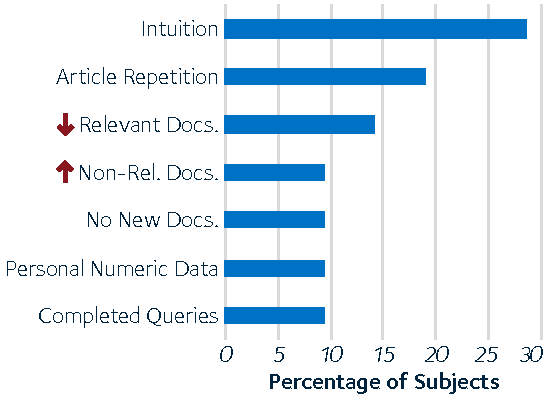
\includegraphics[width=1\textwidth]{figures/ch3-respondents.pdf}
    \end{center}
    \vspace*{-4mm}
    \caption[Responses of a survey by~\cite{dostert2009satisficing}]{Responses of the survey on why subjects stopped by~\cite{dostert2009satisficing}. Like most studies examining stopping behaviour, most subjects stopped because of their \emph{intuition.}}
    \label{fig:stopping_respondents}
\end{wrapfigure}

Indeed, the unarticulated notion of finding \emph{``enough''}~\citep{zach2005enough_is_enough} information links neatly back to the idea of the magnitude threshold stopping heuristic, proposed by~\cite{nickles1995judgment} and detailed in Section~\ref{sec:stopping_background:heuristics:magnitude}. With this heuristic, a searcher would stop once they have accumulated a certain predetermined amount of information. From the results of their study,~\cite{dostert2009satisficing} hypothesised that the threshold was reached once they felt they had correctly identified \emph{half} of the relevant documents available to them. In reality however, the searchers had on average only managed to correctly identify $7.35\%$. In addition to comparisons to the magnitude threshold stopping heuristic,~\cite{dostert2009satisficing} also drew comparisons from their results to the difference threshold stopping heuristic, as outlined in Section~\ref{sec:stopping_background:heuristics:difference}. Recapping, this heuristic considered a searcher's tolerance to not learning anything new -- this is argued by the authors as a reason for respondents citing repetition in the documents found, or a lack of new documents. Lastly, the representational stability stopping heuristic as detailed in Section~\ref{sec:stopping_background:heuristics:representational} was also noted by the authors. With this heuristic concerned with the searcher's underlying mental model of the topic stabilising, the authors noted that evidence for this was shown from subjects responding that a decreasing in relevant documents and an increase in non-relevant documents.

These stopping heuristics were also investigated by~\cite{browne2004stopping_rules} and~\cite{pitts2004stopping_rules} with systems analysts during the process of information requirements determination. The analysts were tasked to gather a series of requirements until they had acquired enough information to draw diagrams of an online grocery shopping system. It was found by~\cite{browne2004stopping_rules} that more experienced analysts tended to use the mental list and magnitude threshold stopping heuristics, with less experienced analysts employing the difference threshold and representational stability stopping heuristics. In addition to these findings, the authors noted that the applicability of different stopping heuristics resulted in varying degrees of quantity, depth and the quality of information obtained.

\subsection{Considering Search Depths}
A number of additional user studies have also considered the so-called \emph{search depth} -- that is, the depth on a list of ranked results that searchers stop clicking (the \emph{click depth}). Studies such as the seminal work by~\cite{cutrell2007eye_tracking} undertook an eye tracking study, and reported that subjects examined the first eight results before deciding to carry out a query reformulation.~\cite{lorigo2008eye_tracking} also examined their subjects' scan paths as they undertook search tasks. On average, subjects scanned only $3.2$ distinct search results per query. This work was supplemented by~\cite{huang2011no_clicks}, where they found that subjects proceeded to issue a new query after inspecting the top four results of the presented~\gls{acr:serp}.

\begin{wrapfigure}[9]{r}{0.45\textwidth}
    \begin{center}
    \vspace*{-2mm}
    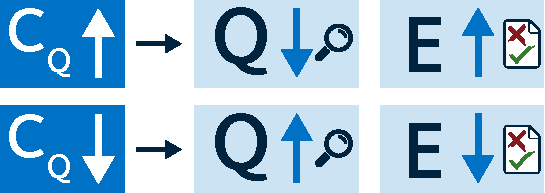
\includegraphics[width=1\textwidth]{figures/ch3-query-cost.pdf}
    \end{center}
    \vspace*{-4mm}
    \caption[The cost-interaction hypothesis]{The \emph{cost-interaction hypothesis}~\citep{azzopardi2011economics}. As the cost of querying increases (\emph{C\textsubscript{Q}}), searchers will issue fewer \textbf{Q}ueries and \textbf{E}xamine more documents per query.}
    \label{fig:query_cost}
\end{wrapfigure}

A study by~\cite{azzopardi2013query_cost} also found that the depth to which subjects examined content was affected by the \emph{cost} of entering a query. With a search interface where subjects were required to invest more effort to enter a query, significantly fewer queries were issued, with the results for these queries examined to greater depths. This was in contrast to subjects who used a standard search interface, where more queries were issued, with subjects examining content to shallower depths. These findings comply with the \emph{query-cost hypothesis}~\citep{azzopardi2011economics}, that states that \emph{as the cost of querying increases, searchers will pose fewer queries and examine more documents per query,} as illustrated in Figure~\ref{fig:query_cost}. Evidence from this study also demonstrated that the search interface searchers are subjected to impacts upon their stopping decision making.

\section{Chapter Summary}
